\section{Acquisition}

\section{Maximizing Light Scattered Towards Camera}

\section{Illumination Polarization}
The Verdi output beam is linearly polarized and passed through single-mode (SM) fibers prior to illuminating scattering samples with the resulting beam having an unknown polarization state due to use of non-polarization-maintaining fibers. This raises several questions 1) What is the beam's polarization state?; 2) Is it constant?; and 3) What is the optimal polarization state of the output beam to maximize light transmission into the sample?

Literature suggests the output beam will have an elliptical polarization state (1) that is variable/unstable (2) due to variable birefringence induced in SM fibers caused by variable internal stresses and temperature fluctuations.

The output polarization state's stability was characterized by placing a power meter photodiode with a static LPF to measure the power of a collimator on the dual collimator stand attached to the RT-5 rail. The measured power for 10 sweeps of the RT-5 through a range of 280 degrees is shown in Figure \ref{fig:lpfpwr_RT5}. There is a clear relationship between the measured power through an LPF and the RT-5 stage position which suggests the polarization state does not remain constant across illumination angles. The ellipticity was not investigated due to requiring a circular polarizing filter (CPF). Fluctuations in measured power across sweeps was due to insertion losses caused by motion of unstable FC/PC fiber connectors on the RT-5 rail. Fixing those connectors to the rail saw significant reductions in fluctuations.

\begin{figure}
    \centering
    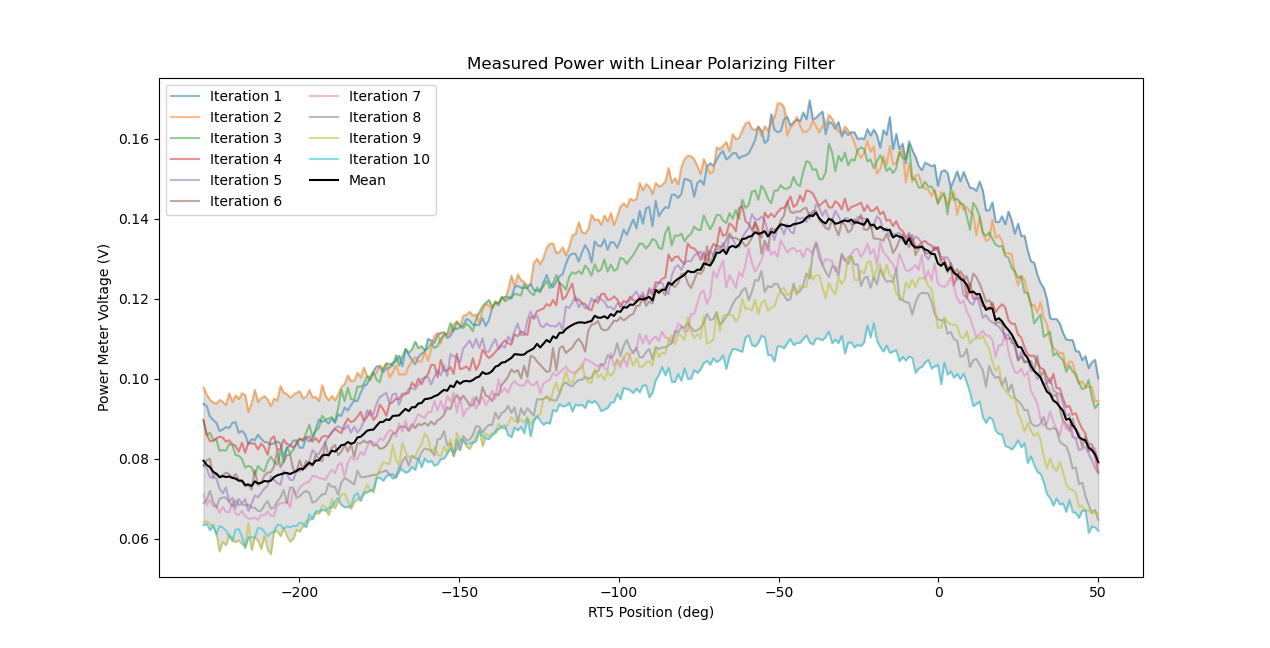
\includegraphics[width=\linewidth]{figures/LPFpwr_vs_RT5.png}
    \caption{}
    \label{fig:lpfpwr_RT5}
\end{figure}

Polarization state for Figure \ref{fig:lpfpwr_RT5}:
\begin{itemize}
    \item $S_0 = 0.200696$
    \item $S_1 = -0.028441$
    \item $S_2 = 0.06834$
    \item $S_DoP = \sqrt{S_1^2 + S_2^2}/S_0 \approx 0.37$
\end{itemize}


\subsection{Optimizing Illumination \& Sample Orientation to Maximize Light Transmission}
Given a linearly polarized illumination laser beam, an acquisition sensor offset by some scattering angle, and a scattering sample inside a glass cell, the goal is to determine 1) the optimal sample orientation and 2) the optimal angle of polarization to maximize light transmitted from the illuminator to the acquisition sensor.

\subsubsection{Fresnel Formulae}
The contents in this section are paraphrased from \cite{born2013principles}. Consider a plane wave with amplitude A incident on a surface. The electric and magnetic field vectors can be decomposed into two components parallel and perpendicular to the surface plane. The incident electric field is

\begin{equation}
    E^{(i)} = 
    \begin{bmatrix}
        -A_{||} \cos{\theta_i} e^{-i \tau_i} \\
        A_\perp e^{-i \tau_i} \\
        A_{||} \sin{\theta_i} e^{-i \tau_i}
    \end{bmatrix}
\end{equation}

where $E_x, E_z$ are in the plane, and $E_y$ is along the plane normal. The complex exponential argument is defined

\begin{equation}
    \tau_i = \omega \big( t - \tfrac{\mathbf{r}^\intercal \mathbf{s^{(i)}}}{v} \big) = \omega \big( t - \tfrac{x \sin{\theta_i} + z \cos{\theta_i}}{v} \big)
\end{equation}

The magnetic field vector $H$ is written similarly through the relation $H = \sqrt{\epsilon} \mathbf{s} \times \mathbf{E}$.
where $\mathbf{s}$ is the light's velocity vector. If $T$ and $R$ denote the transmitted and reflected amplitudes, then the transmitted field is

\begin{equation}
    E^{(t)} = 
    \begin{bmatrix}
        -T_{||} \cos{\theta_t} e^{-i \tau_t} \\
        T_\perp e^{-i \tau_t} \\
        T_{||} \sin{\theta_t} e^{-i \tau_t}
    \end{bmatrix},
\end{equation}

and the reflected field is

\begin{equation}
    E^{(r)} = 
    \begin{bmatrix}
        -R_{||} \cos{\theta_r} e^{-i \tau_r} \\
        R_\perp e^{-i \tau_r} \\
        R_{||} \sin{\theta_r} e^{-i \tau_r}
    \end{bmatrix}.
\end{equation}

The tangential components of the electric and magnetic fields must be continuous across the boundary, resulting in four boundary conditions:

\begin{align}
    E^{(i)}_x + E^{(r)}_x = E^{(t)}_x \quad & E^{(i)}_y + E^{(r)}_y = E^{(t)}_y \\
    H^{(i)}_x + H^{(r)}_x = H^{(t)}_x \quad & H^{(i)}_y + H^{(r)}_y = H^{(t)}_y
\end{align}

These boundary conditions can be solved for an expression of the transmitted and reflected amplitudes components by using the Maxwell relation $n = \sqrt{\epsilon}$

\begin{align}
    T_{||} = \frac{2 n_1 \cos{\theta_i}}{n_2 \cos{\theta_i} + n_1 \cos{\theta_t}} A_{||} \quad &
    T_{\perp} = \frac{2 n_1 \cos{\theta_i}}{n_1 \cos{\theta_i} + n_2 \cos{\theta_t}} A_{\perp} \\
    R_{||} = \frac{n_2 \cos{\theta_i} - n_1 \cos{\theta_t}}{n_2 \cos{\theta_i} + n_1 \cos{\theta_t}} A_{||} \quad &
    R_{\perp} = \frac{n_1 \cos{\theta_i} - n_2 \cos{\theta_t}}{n_1 \cos{\theta_i} + n_2 \cos{\theta_t}} A_{\perp}
\end{align}

\subsubsection{Effects of Polarization on Fresnel Formulae}
The light intensity is

\begin{equation}
    S = \frac{c}{4\pi} \sqrt{\epsilon} E^2 = \frac{cn}{4\pi} E^2
\end{equation}

The resulting energy incident on a surface with unit area $A$ is

\begin{equation}
    J^{(i)} = S^{(i)} \cos{\theta_i} = \frac{cn_1}{4\pi} |A|^2 \cos{\theta_i}
\end{equation}

with reflected and transmitted energies

\begin{align}
    J^{(r)} = \frac{cn_1}{4\pi} |R|^2 \cos{\theta_i} & \quad and \quad J^{(t)} = \frac{cn_2}{4\pi} |T|^2 \cos{\theta_t}.
\end{align}

The reflectivity and transmissivity are

\begin{align}
    \mathcal{R} = \frac{J^{(r)}}{J^{(i)}} = \frac{|R|^2}{|A|^2} & \quad and \quad \mathcal{T} = \frac{J^{(t)}}{J^{(i)}} = \frac{|T|^2}{|A|^2}
\end{align}

which satisfy the law of conservation of energy by summing to 1

\begin{equation}
    \mathcal{R} + \mathcal{T} = 1.
\end{equation}

The reflectivity and transmissivity are functions of polarization with respect to the parallel and perpendicular directions. If the incident electric field $\mathbf{E}$ makes an angle $\alpha_i$ with respect to the plane, the parallel and perpendicular area components are

\begin{align}
    A_{||} = A \cos{\alpha_i} & \quad and \quad A_{\perp} = A \sin{\alpha_i}
\end{align}

The parallel energy component of the incident light is

\begin{align}
    J_{||}^{(i)} &= \frac{cn_1}{4\pi} |A_{||}|^2 \cos{\theta_i} \nonumber \\
    &= \frac{cn_1}{4\pi} |A |^2 \cos^2{\alpha_i} \cos{\theta_i} \nonumber \\
    &= J^{(i)} \cos^2{\alpha_i}
\end{align}

with that of the perpendicular component following similarly:

\begin{equation}
    J_{\perp}^{(i)} = J^{(i)} \sin^2{\alpha_i}.
\end{equation}

The reflectivity in terms of polarized light is

\begin{align}
    \mathcal{R} = \frac{J^{(r)}}{J^{(i)}} &= \frac{J_{||}^{(r)} + J_{\perp}^{(r)}}{J^{(i)}} \nonumber \\
    &= \frac{J_{||}^{(r)}}{J_{||}^{(i)}} \cos^2{\alpha_i} + \frac{J_{\perp}^{(r)}}{J_{\perp}^{(i)}} \sin^2{\alpha_i} \nonumber \\
    &= \mathcal{R}_{||} \cos^2{\alpha_i} + \mathcal{R}_{\perp} \sin^2{\alpha_i},
\end{align}

and the transmissivity is

\begin{equation}
    \mathcal{T} = \mathcal{T}_{||} \cos^2{\alpha_i} + \mathcal{T}_{\perp} \sin^2{\alpha_i}.
\end{equation}

Reflectivity and transmissivity must satisfy conservation of energy respectively:

\begin{equation}
    \mathcal{R}_{||} + \mathcal{T}_{||} = 1, \qquad \mathcal{R}_{\perp} + \mathcal{T}_{\perp} = 1.
\end{equation}

When light is incident normal to the surface, $\alpha_i = 0$ for all E-field orientations, meaning there is no distinction between the parallel and perpendicular components, and the reflectivity and transmissivity are written

\begin{equation}
    \mathcal{R} = \bigg(\frac{n - 1}{n+1} \bigg)^2, \qquad \mathcal{T} = \frac{4n}{(n + 1)^2}
\end{equation}

where $n = n_2 / n_1$.

\subsubsection{Fresnel Relations as Mueller Matrices}
\paragraph{Transmission}


\paragraph{Scattering}
This section summarizes the results in \cite{bohren2008absorption}. Assuming light with wavevector $k$ is scattered from a small sphere with radius $a$ with scattering amplitude coefficient $a_1 \in \mathbb{C}$, the scattered field at distance $r$ from the scatterer, the Mueller matrix is

\begin{equation}
    \Mv_s = \frac{9|a_1|^2}{4k^2r^2}
    \begin{bmatrix}
        \tfrac{1}{2}(1 + \cos^2{\theta}) & \tfrac{1}{2}(\cos^2{\theta} - 1) & 0 & 0 \\
        \tfrac{1}{2}(\cos^2{\theta} - 1) & \tfrac{1}{2}(1 + \cos^2{\theta}) & 0 & 0 \\
        0 & 0 & \cos{\theta} & 0 \\ 
        0 & 0 & 0 & \cos{\theta}
    \end{bmatrix}
\end{equation}

where the scattering coefficient is defined

\begin{equation}
    a_1 = -\frac{i2x^3}{e} \frac{m^2 - 1}{m^2 + 2} - \frac{i2x^5}{5} \frac{(m^2 - 2)(m^2 - 1)}{(m^2 + 2)^2}
\end{equation}

with scale factor and relative refractive index

\begin{equation}
    x = ka = \frac{2 \pi N a}{\lambda},  \qquad m = \frac{N_1}{N} = \frac{k_1}{k}
\end{equation}

where $N$ and $N_1$ are the medium's and particle's refractive indices respectively. The scattering Mueller matrix is defined within the scattering plane containing the incoming and outgoing directions as well as the scattering particle.

\subsubsection{Simulation Results}
 
\paragraph{Unpolarized Beam}
% Plots will be called polctrl0_traj and polctrl0_trans

\paragraph{Linearly Polarized Beam}

\begin{figure}
    \centering
    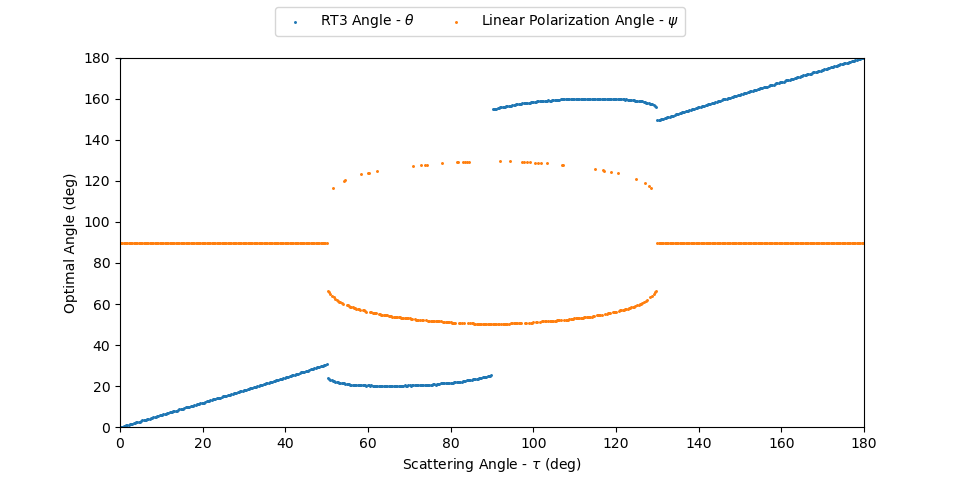
\includegraphics[width=0.49\linewidth]{figures/polctrl1_traj.png}
    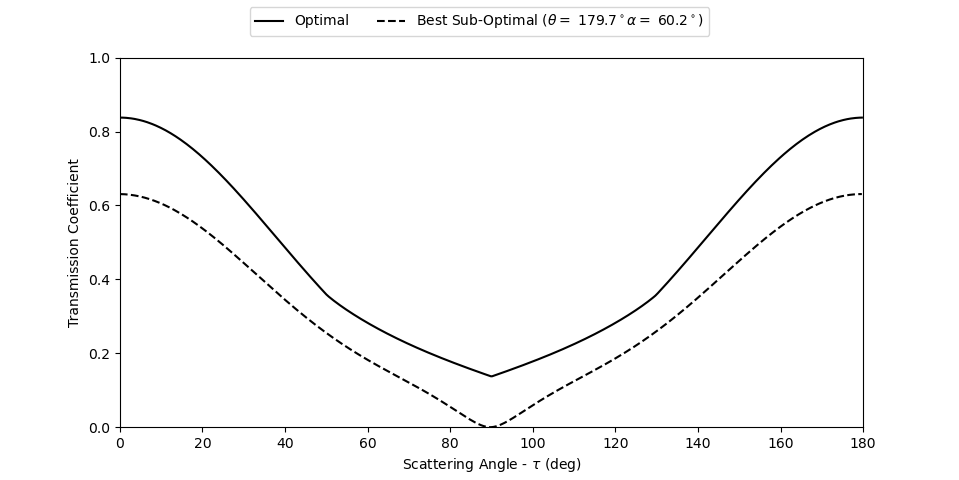
\includegraphics[width=0.49\linewidth]{figures/polctrl1_trans.png}
    \caption{}
    \label{fig:polctrl1}
\end{figure}

\subsection{Simulation}

\subsection{Depolarizer Spatial Characterization}
One option is to depolarize the illumination beams via Thorlabs DPP25-A liquid crystal polymer depolarizer. This optic is a series of linear polarizing strips each oriented in 45-degree increments. The incident beam is passed through these strips, and the output beam is a combination of linear polarization states with different angles of polarization. Since strips are distributed spatially, the output beam's polarization state is a function of the incident beam size.

\begin{figure}
    \centering
    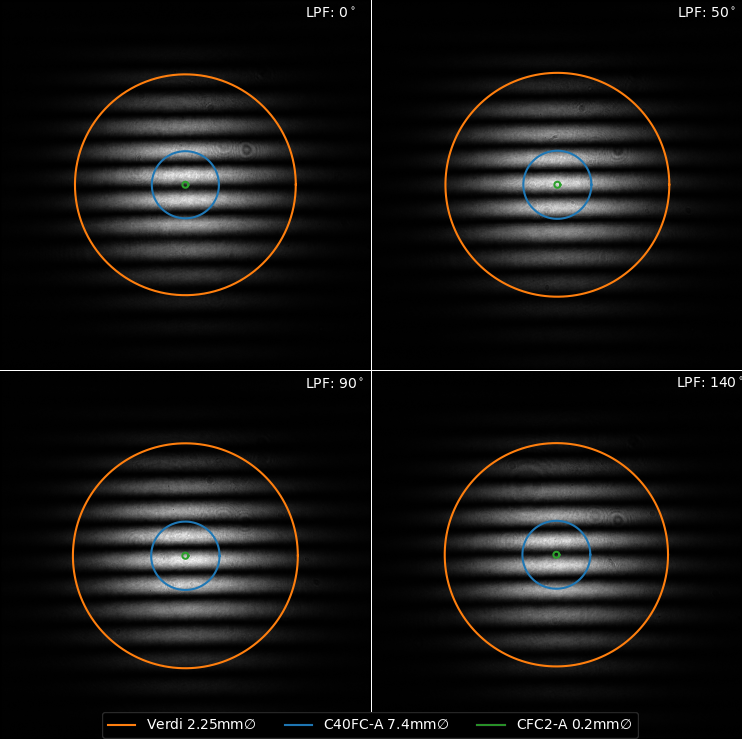
\includegraphics[width=0.5\linewidth]{../figures/depol_spatial.png}
    \caption{}
    \label{fig:depol_spatial}
\end{figure}

The effect of beam size on output polarization state was characterized by measuring the spatial distribution of polarization state using a camera. The Verdi output beam was coupled into a 2-meter single-mode fiber whose output was collimated using Thorlabs C40FC-A. That beam was passed through the depolarizer mounted on Thorlabs CRM1PT followed by a linear polarizing filter mounted on Thorlabs CRM1T. The beam was then passed through an ND=2.0 filter prior to measurement by the camera. The camera was Grasshopper3 GS3-PGE-91S6M with a Leica Summicron-A 50mm 1:2 lens focused at its shortest working distance (1:6.6 magnification). Acquisition consisted of rotating the LPF in 10-degree increments over a range of 170 degrees and acquiring a 16-bit image for each LPF orientation.

The intensity profiles of the depolarized beam for four LPF orientations is shown in Figure \ref{fig:depol_spatial}. Each profile is a Gaussian-enveloped sinusoid whose phase changes with the LPF orientation. Each image is overlaid with 1/$e^2$ beam diameters for two collimators' output beams and the Verdi output beam. The C40FC-A and Verdi beam profiles are large enough to cover at least a full period of the depolarizer's structure, while the CFC2-A beam does not. Therefore, the depolarizer would not be effective if used with the CFC2-A collimator.
